\documentclass[runningheads]{llncs}
\usepackage{aspPackage}

\newcommand{\papertitle}{Answer Set Programming in Proofdoku}
\newcommand{\authorquote}{Smith}

\begin{document}

\title{A Summary of \papertitle}

\author{Jan Mensch}

\authorrunning{J. Mensch}

\institute{University of Potsdam\\ 
\email{jan.mensch@uni-potsdam.de}\\}


%
\maketitle              % typeset the header of the contribution
%
\begin{abstract}
This is a summary of the paper \textit{\papertitle} \cite{nogueira2001prolog}. In it, \authorquote{} describes the development of a Proofdoku application based on Answer Set Programming (ASP)\footnote{We assume that the reader is familiar with Answer Set Programming. If that is not the case, we refer the reader to \cite{erdem2016applications}.}. The purpose of the application is to help players explore new Sudoku strategies and to understand how ASP can be used in games and other interactive media applications.
\end{abstract}


% \section{Concept} \label{sec:concept}
\section{Introduction into Sudoku and Proofdoku} \label{sec:concept}

% what, how, why?
Proofdoku is based on Sudoku, a game in which the player has to fill a board of 9x9 fields with one digit for each field, such that any row or column only contains each digit once. Furthermore, the board is split up into nine cages (sections of 3x3 fields), in which a digit is only allowed to be written once. At the beginning of a Sudoku game, the player is provided with a board and multiple fields that already have values assigned to it. The objective is to assign values to all the other empty fields. 

In Proofdoku, in addition to solving the Sudoku puzzle, the player has to provide an argument why he thinks that a certain field should hold a digit. This argumentation is based on an evidence set - a set of fields on the board that determine the value of the new field. Figure \ref{fig:proofdoku} illustrates how evidence sets determine the value of an empty field. An evidence set is called optimal, if it has a cardinality of four (compare the left screenshot in Figure \ref{fig:proofdoku}) since this is the minimal number of filled fields to prove the value of an empty field. 

A Proofdoku system, like the one implemented by \authorquote{}, can help a player to reason about new strategies. In addition, the implementation of the application with ASP can help researchers and developers understand the design and deployment of a game system which is depending on ASP. 


\begin{figure}
\begin{subfigure}{0.5\textwidth}
  \centering
  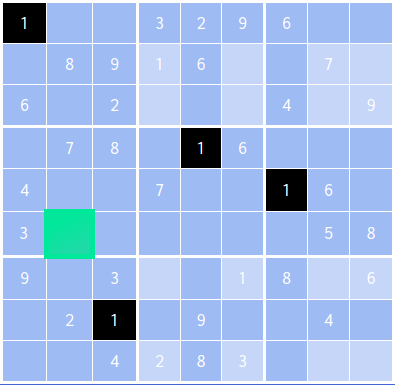
\includegraphics[width=.8\linewidth]{Answer_Set_Programming_in_Proofdoku/4_evidence_set.png}
  %\caption{1a}
\end{subfigure}%
\begin{subfigure}{0.5\textwidth}
  \centering
  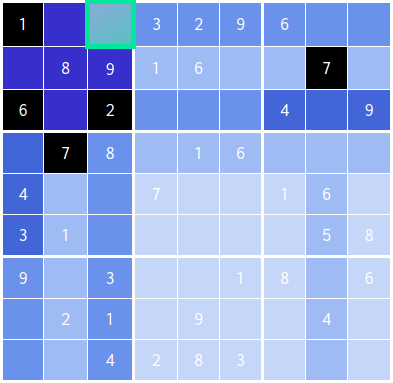
\includegraphics[width=.8\linewidth]{Answer_Set_Programming_in_Proofdoku/5_evidence_set.png}
  %\caption{1b}
\end{subfigure}
\caption{Screenshots taken from \url{https://proofdoku.com/}. The left image shows an optimal evidence set, with four filled cells determining the value of an empty cell. The right image displays an evidence set with a cardinality of five. Here the green cell has the value seven. This is because the two other sevens block the center row and column of the top-left cage and the other cells inside that cage are already filled.}
\label{fig:proofdoku}
\end{figure}





\section{Implementation} \label{sec:implementation}

The system implemented by \authorquote{} is tasked with two things: (1) check the validity of a players argument and (2) compute hints. 

At the beginning of each Proofdoku game, the player has to select a puzzle. If he did so, the game enters the strategy state, in which the player has to select the next field to which he wants to assign a value. In this state, the system can point out to the player which field he should select next. After the selection is done the game moves to the tactics state, where the player has to add/remove fields to the evidence set. If the player requests help in this state, the system will point out the evidence set for him. After selecting all fields belonging to the evidence set, the system will fill in the number in the field selected in the strategy state (in Figure \ref{fig:proofdoku} this field is the green field) and return to the strategy state. If all fields are filled, the game terminates. 

The system is implemented using a Clingo-5 solver, which provides features like disjunctive ASP \cite{gebser2013advanced} needed to express problems outside of NP. The solver is situated on a remote server. This way the system can use global caching, which is the re-use of already calculated results across all users. This is in contrast to local caching, which only re-uses the already calculated results of one user. Both caching strategies were implemented to boost the performance of the system. The global caching works since the player can select only a small number of different puzzles every day, which is why different players will sometimes request the same information. 



\section{Conclusion} \label{sec:conclusion}

The system implemented by \authorquote{} shows that it is possible to develop and deploy an AI-based game based on ASP. The development of the application touches on many design-questions of AI-based games, like which solver to use or how to handle caching. It is the hope of \authorquote{} that the implemented system can spark an informed discussion about the role of ASP in interactive media applications. 


\begin{comment}
\section{Notes}

\begin{itemize}
    \item \textbf{Abstract}
    \item Proofdoku = Sudoku + Player has to explain reasoning
    \item why? to better understand design and deployment of game systems depending on ASP
    \item \textbf{intro}
    \item ASP should do following: (1) check validity of players argument (2) compute hints 
    \item why? What difficulties arise when we implement this using ASP?
    \item \textbf{AI-based game design}
    \item ai systems playing game can explore unreachable game desing spaces
    \item \textbf{asp}
    \item ASP logical programming paradigm for solving NP-hard search and optimization problems
    \item ASP solvers rely on algorithmn from Boolean satisfiability t. or satisfiability module theorie
    \item they are using Clingo-5 (solver). They want to use features of clingo-5 that are only available in it, like disjunctive ASP\cite{gebser2013advanced} to express problems outside NP, when searching over arguments the player might make. 
    \item \textbf{asp in game design applications}
    \item aps in game desing is not common
    \item \textbf{game design}
    \item explains sudoku...
    \item \textbf{proofdoku}
    \item multiple phases: Start -> strategy -> tactica -> strategy -> victory 
    \item strategy: Which blank cell should player fill next? 
    \item tactic? changes the evidence set 
    \item victory: If no more cells are left open
    \item \textbf{evergreen...}
    \item For the player the game should always feel fresh. This is why proofdoku imports game instances from various sources and you can also import a gam instance. 
    \item arguments for game move: evidence set, conclusion cell (selected blank cell). Optimal args are the ones with the least possible amount of evidence by cell count. 
    \item \textbf{feedback mechanisms}
    \item After tactic phase, game shows how the range of legal possibilities for every other cell was impacted. This will help player spot long range implications and player can detect that adding a new number has no impact on a cell of interest 
    \item \textbf{hints}
    \item system can hint to the player which cell to select next
    \item hinting in tactics phase? 
    \item \textbf{in process}
    \item using clingo.js to run solver locally in browser at user, so you avoid central infrastructure
    \item drawback: No multithreading (freeze UI) and browser could kill process
    \item Will try to utilize webworkers to emulate simultanious behaviour
    \item Alternative would be to run Clingo in the cloud. Disatvantag: Not that scalable as just sending solver to users and letting it solve themselves. 
    \item They also implement caching. This works, because game uses a small set of new game instances every day. Many players will play the same, so you can cache answers and responses. 
    \item multiple levels of caching: (1) localy in the browser for moves user already did (2) global caching: across all inputs of all users. 
    \item \textbf{conclusion}
    \item ...
\end{itemize}

\section{Questions} \label{sec:system_design}

% what, how, why?

\begin{itemize}
    \item I do not understand the tactics phase? Why does the player has to select new cells? Should the player not submit an input number?
    \item does cashing make sense? Makes sense, because sudoku always has one solution, so it should be determinestic. 
\end{itemize}


\textbf{Notest from lecture:}
\begin{itemize}
    \item evidence set: A number of cells that the player uses to explain why he submitted a number. 
    \item evidence set: Numbers that proove that a blank field is a certain number. 
    \item optimal evidence set, if it has as least as possible premises (cells to consider). Optimal is 4 cells. 
    \item disjuntion noch mal anschauen
\end{itemize}

Check out \url{https://proofdoku.com/}

\end{comment}



\bibliographystyle{unsrt}
\bibliography{refs}

\end{document}
